\chapter{Introduction}
\label{chp:intro}
\epigraph{``First things first, but not necessarily in that order.''}{The Fourth Doctor, Doctor Who: Megalos (1980)}
\section{Introduction}

\subsection{Neutrino Physics}

There are a plethora of physics phenomenon in which neutrinos are involved, including beta decay, fusion, and supernovae. As part of the Standard Model, they are descibed as being Dirac fermions with no electric charge with three flavours: the electron neutrino, the muon neutrino and the tau neutrino, corresponding with their associated leptons: the electron, muon and tauon. Prior to the discovery of neutrino oscillations, it was believed that neutrinos were massless, but they in fact have small but non zero masses ($\le$ 1eV) \cite{Aker_2019}. This chapter will discuss a brief history of neutrino physics including the discovery of neutrino oscillations, the manner in which neutrinos interact with nuclei in the Super-Kamiokande detector, and the motivation behind an NCQE neutron tagging analysis.

\subsection{History of Neutrino Physics}

To correct a violation of energy and momentum conservation discovered in beta-decay, Wolfgang Pauli put forward the idea of a neutrino as a solution \cite{brown_idea_1978}.  He originally named this particle the ``neutron'', prior to Chandwick's discovery of the actual neutron two years later.  Enrico Fermi then proposed to call it the neutrino, Italian for ``little neutral one". In 1934, Enrico Fermi's theory of beta decay stated that a neutron could decay to a proton, electron and an antielectron neutrino \cite{bethe1934neutrino} and in 1956 \cite{luca_electroweak}, Clyde Cowan and Frederick Reines directly confirmed the existence of neutrinos \cite{cowan_reines}, by detecting the electron antineutrino originating from inverse beta decay produced from nuclear reactor or fission products. In inverse beta decay an electron antineutrino interacts with a proton to produce a neutron and positrons \cite{vogel1999angular}.
\newline
These positrons pair-annihilate with electrons and produce two 0.5 MeV gamma rays and scintillator material was placed in a tank of water, which was used to detect the gamma photons, and the scintillator light produced flashes of visible light which were detected by photomultiplier tubes. Cadmium chloride was used to detect the coincident neutron, which after exciting and de-exciting, emits a gamma ray within 5 microseconds after the pair-annihilation gammas are detected \cite{reines1956neutrino}. In 1962, Ledermen, Schwartz and Steinberger detected the muon neutrino \cite{feinberg1963physics}, \cite{lederman_schwartz}. To discover the muon neutrino, the AGS (Alternating Gradient Synchroton) at Brookhaven \cite{courant1958theory} was used - the AGS's beam of protons was used to produce a shower of pions after slamming into a beryllium target. These pions would travel toward a 5,000-ton steel wall (constructed from old battleship plates! \cite{ricoux2010search}) and they would decay into muons and neutrinos, but only neutrinos would be able to pass through the steel wall into a spark chamber filled with neon. As neutrinos coursed through this chamber, one neutrino would ocassionally hit a proton in an aluminium nucleus which would produce muon tracks, instead of the showers produced from electrons, proving that there were muon neutrinos in the neutrinos that passed through the chamber \cite{lindley2015landmarks}. 
\newline

In 2000 the DONUT collaboration (Direct Observation of NU Tau) at Fermilab detected the existence of the tau neutrino \cite{kodama2001observation}. A beam of neutrinos (which they expected to contain tau neutrinos) was fired at iron plates with alternating layers of emulsion, and very very small number of these tau neutrinos interacted with an iron nucleus to produce the tau lepton, which decayed leaving a track in the emulsion \cite{kodama2004identification}. These tracks contained a kink, which were a sign of the tau neutrino, and only four such tracks were detected out of a possible six million \cite{kodama1993muon}.

\subsection{The Solar Neutrino Problem}

The Standard Solar Model predicts that most of the solar neutrino flux (about 90\%) come from the proton-proton chain reaction \cite{borexino2018comprehensive}, where the solar neutrinos produced have energies below 0.4 MeV. Figure \ref{fig:ppchain} shows the processes which make up the pp chain, along with the branching percentages where it produces a neutrino. 

\begin{figure}
    \centering
    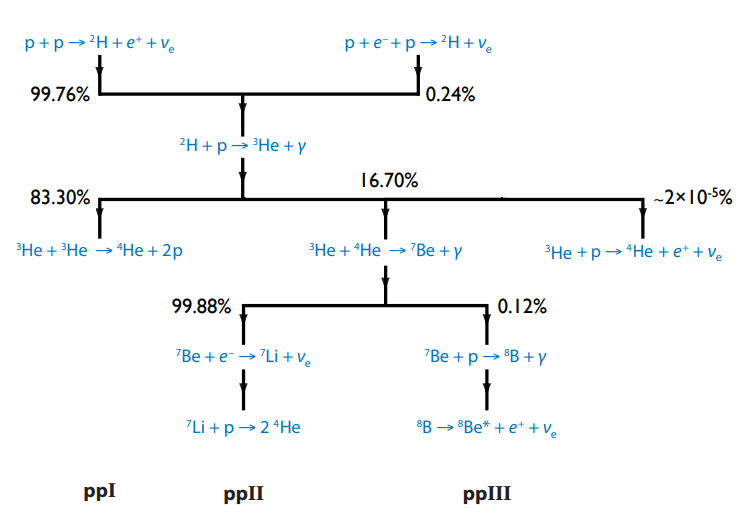
\includegraphics[width=\textwidth]{Figures/ppchain.png}
    \caption{Proton-proton chain cycle with branching percentages shown}
    \label{fig:ppchain}
\end{figure}

Only experiments that use Gallium can detect neutrinos with this energy, whereas experiments whose detector medium is Chlorine can observe neutrinos from ${ }^{7} \mathrm{Be}$ (production equation of which is shown in Figure \ref{fig:ppchain}). Experiments whose detector medium is water (such as Super-Kamiokande and SNO) can only see the ${ }^{8} \mathrm{B}$ neutrinos, as shown in Figure \ref{fig:nu_energy_bachall}.

\begin{figure}
    \centering
    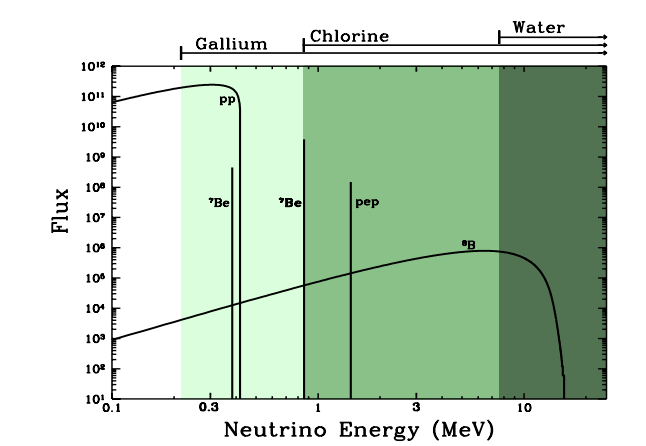
\includegraphics[width=\textwidth]{Figures/nu_energy_bachall.png}
    \caption{Solar neutrino fluxes predicted by Bachall's Standard Solar Model, and which experiments are able to detect them \cite{Bahcall_2003}.}
    \label{fig:nu_energy_bachall}
\end{figure}

In the 1960s, the Homestake experiment made the first measurement of solar electron neutrino flux \cite{homestake_davis}. The experiment used a perchloroethlene-based detector, placed 1,478 metres underground in the Homestake Gold Mine in South Dakota. When an electron neutrino interacts with ${ }^{37} \mathrm{Cl}$ in the perchloroethlene, the ${ }^{37} \mathrm{Cl}$ becomes a radioactive isotope of ${ }^{37} \mathrm{Ar}$ which is extracted by bubbling helium through the tank, and then counted in order to determine how many neutrinos had been captured \cite{davis1994review}. The theoretical solar neutrino flux calculated by John Bachall was about three times as much as Raymond Davis' results from the experiment: with Bachall's calculations predicting a solar neutrino flux of $8.1 \pm 1.2$ SNU, whereas the Homestake experimental results showed a flux of $2.56 \pm 0.25$ SNU \cite{JKonijn1999}. These results were consistent with those from the subsequent Kamiokande, SAGE and GALLEX experiments. Super-Kamiokande's main detection channel for solar neutrinos is the elastic-scattering channel, which has a minimum energy threshold value (recoil electron kinetic energy) of 5 MeV. In this channel, Super-Kamiokande observed a solar neutrino capture rate of $0.45 \pm 0.02$ SNU, while the solar neutrino model prediction was $1.0 \pm 0.2$ SNU. Turning our attention to the results of the Gallium experiements, namely SAGE and GALLEX, they also showed a discrepancy regarding the solar model predictions. Due to their sensitivity to the bulk of the proton-proton chain neutrino flux, they have a larger solar neutrino capture flux rate, with SAGE observing $70.8 \pm 5.0$ SNU, and GALLEX observing $77.5 \pm 8.0$ SNU, while the model prediction was $129 \pm 9.0$ SNU, a difference of about 40\%. This discrepancy of experimental results compared with the Standard Solar Model prediction became known as the Solar Neutrino Problem \cite{Haxton_1995}. 

The way to combat this discrepancy and prove that the cause of the Solar Neutrino Problem was neutrino oscillations was finding a way to detect solar neutrino flux which was not dependent on neutrino flavour. Due to these experiments only detecting solar neutrinos through charged current interactions, they wouldn't be able to detect muon or tau neutrinos. However, with the Sudbury Neutrino Observatory (SNO) experiment this would change, as SNO used heavy water $D_{2}O$ as its detector medium. Deuteron consists of a proton and a neutron and due to how little energy it takes to break it apart (2.2 MeV), an electron, muon or tau neutrino can very easily break it apart, so that SNO can detect the final state neutron then muon and tau neutrinos would be visible to the detector. The three main channels SNO uses to detect neutrinos is the elastic scattering channel, the charged current channel, and the neutral current channel. Elastic scattering allows SNO to see muon and tau neutrino flux given by $\phi(\nu_{e} + 0.15(\phi(\nu_{\mu}) + (\nu_{\tau})))$. The most important neutrino interaction channel regarding SNO being able to measure the muon and tau neutrino flux is the neutral current (NC) channel (shown in Equation \ref{eq:neutral_current_SNO}), as it allows SNO to measure the total flux \cite{krastev2002global}.

\begin{equation}
    \nu + d \rightarrow n + p + \nu
\label{eq:neutral_current_SNO}
\end{equation}

Using these two reaction channels, along with the charged current channel (CC), which can only measure electron neutrino flux, SNO was able to measure the individual neutrino flavour fluxes, shown in Equation \ref{eq:neutrino_flux_SNO}. 


\begin{align}
&\phi_{C C}=\phi\left(\nu_{e}\right)=1.76 \pm 0.01 10^{-8} \mathrm{~cm}^{-2} \mathrm{~s}^{-1} \label{eq:neutrino_flux_SNO}\\
&\phi_{E S}=\phi\left(\nu_{e}\right)+0.15\left(\phi\left(\nu_{\mu}\right)+\phi\left(\nu_{\tau}\right)\right)=2.39 \pm 0.26 10^{-8} \mathrm{~cm}^{-2} \mathrm{~s}^{-1} \notag\\
&\phi_{N C}=\phi\left(\nu_{e}\right)+\phi\left(\nu_{\mu}\right)+\phi\left(\nu_{\tau}\right) = 5.09 \pm 0.63 10^{-8} \mathrm{~cm}^{-2} \mathrm{~s}^{-1} \notag
\end{align}


From Equation \ref{eq:neutrino_flux_SNO}, you can see that the flux of muon and tau neutrinos from the Sun is $\phi(\nu_{\mu}) + (\nu_{\tau}) - \phi(\nu_{e}) = 3.33 \pm 0.62$ , which is 3 times that of the value for $\phi(\nu_{e})$, and as we know that the Sun only produces $\nu_{e}$, it means that the neutrinos must be changing flavour to mu and tau neutrinos on their journey to Earth, definitely solving the solar neutrino problem. 


\subsection{Neutrino Oscillation Theory}
In 1957, Bruno Pontecorvo postulated that neutrinos could transition from neutrinos to antineutrinos and vice versa (similarly to how two kinds of neutral kaons $\bar{K_{0}}$, and $K_{0}$ were found to oscillate) \cite{Pontecorvo:1957cp}. Neutrino flavour oscillation theory was then developed by Maki, Nakagawa and Sakata in 1962. The PMNS matrix (Pontecorvo-Maki-Nakagawa-Sakata matrix) is the neutrino analogue of the Cabbibo-Kobayashi-Masakawa quark mixing matrix \cite{maki_pmns}, and is shown in Equation \ref{eq:neutrino_osc} as $\boldsymbol(U_{\alpha i}^{*})$ which shows the relationship between the mass and flavour eigenstates for a neutrino with a definite flavour of $\alpha$ and a definite mass of $m_{i}$.


\begin{align}
&\left|\nu_{\alpha}\right\rangle=\sum_{i} \boldsymbol{U_{\alpha i}^{*}}\left|\nu_{i}\right\rangle \label{eq:neutrino_osc}  \\
&\left|\nu_{i}\right\rangle=\sum_{\alpha} \boldsymbol{U_{\alpha i}}\left|\nu_{\alpha}\right\rangle \notag
\end{align}


In Equation \ref{eq:neutrino_osc}, the terms $U_{\alpha i}^{*}$ and $U_{\alpha i}$ are the complex conjugate and normal PMNS matrix. Equation \ref{eq:PMNS_matrix} shows the 3x3 form of the PMNS matrix, where $c_{ij} = cos {\theta_{ij}}$ and $s_{ij} = sin {\theta_{ij}}$.

\begin{align}
&U=\left(\begin{array}{ccc} \label{eq:PMNS_matrix}
1 & 0 & 0 \\
0 & c_{23} & s_{23} \\
0 & -s_{23} & c_{23}
\end{array}\right)\left(\begin{array}{ccc}
c_{13} & 0 & s_{13} e^{-i \delta_{\mathrm{CP}}} \\
0 & 1 & 0 \\
-s_{13} e^{i \delta_{\mathrm{CP}}} & 0 & c_{13}
\end{array}\right)\left(\begin{array}{ccc}
c_{12} & s_{12} & 0 \\
-s_{12} & c_{12} & 0 \\
0 & 0 & 1
\end{array}\right)\\
&=\left(\begin{array}{ccc} \notag
c_{12} s_{13} & s_{12} c_{13} & s_{13} e^{-i \delta_{\mathrm{CP}}} \\
-s_{12} c_{23}-c_{12} s_{13} s_{23} e^{i \delta_{\mathrm{CP}}} & c_{12} c_{23}-s_{12} s_{13} s_{23} e^{i \delta_{\mathrm{CP}}} & c_{13} s_{23} \\
s_{12} s_{23}-c_{12} s_{13} c_{23} e^{i \delta_{\mathrm{CP}}} & c_{12} s_{23}-s_{12} s_{13} c_{23} e^{i \delta_{\mathrm{CP}}} & c_{13} c_{23}
\end{array}\right)
\end{align}



In Equation \ref{eq:PMNS_matrix}, if the sin $\delta_{CP}$ terms are not equal to 0, it means that there will be imaginary terms in the matrix, which will contribute to CP (charge-parity) violation \cite{NUNOKAWA2008338}. The angles $\theta_{12}$, $\theta_{23}$ and $\theta_{13}$ are mixing angles \cite{giganti2018neutrino}.

\subsubsection{Two-flavour neutrino oscillations in vacuum}

If a neutrino is produced in the flavour state $\left|\nu_{\alpha}\right\rangle$ in a vacuum, using the PMNS matrix for the relationship between the mass eigenstate and the flavour eigenstate, propagating the neutrino according to the time-dependent Schrodinger equation with no potential would yield a solution to this equation as a plane wave, shown in Equation \ref{eq:schro_eq_solution}.

\begin{equation}
i \frac{\partial}{\partial t}\left|\nu_{i}(x, t)>=E\right| \nu_{i}(x, t)>=-\frac{1}{2 m_{i}} \frac{\partial^{2}}{\partial x^{2}} \mid \nu_{i}(x, t)>
\label{eq:schro_eq_solution}   
\end{equation}

The solution to Equation \ref{eq:schro_eq_solution} is a plane wave of the form shown in Equation \ref{eq:plane_wave_sol}.

\begin{equation}
\left|\nu_{k}(x, t)>=e^{-i\left(E_{k} t-p_{k} x\right)}\right| \nu_{k}(0,0)>=e^{-i \phi_{k}} \mid \nu_{k}(0,0)>
\label{eq:plane_wave_sol}
\end{equation}

The probability of oscillation to flavour state $\left|\nu_{\beta}\right\rangle$ at time $t$ is given by Equation \ref{eq:transition_prob_nu}. 


\begin{align}
P\left(\nu_{\alpha} \rightarrow \nu_{\beta}\right) &=\left|\left\langle\nu_{\beta} \mid \nu_{\alpha}(t)\right\rangle\right|^{2} \label{eq:transition_prob_nu}\\
&=\sum_{i, j} \boldsymbol(U_{\beta i}^{*})\boldsymbol(U_{\beta i})\boldsymbol(U_{\alpha j})\boldsymbol(U_{\beta j}^{*}) e^{-i\left(E_{i}-E_{j}\right) t} \notag
\end{align}



For a two-flavour oscillation probability calculation, the matrix which transforms a vector in flavour basis into mass basis is simply a 2x2 rotation matrix (where $\theta$ is the mixing angle) so that:

$$
\left(\begin{array}{l}
\nu_{\alpha} \\
\nu_{\beta}
\end{array}\right)=\left(\begin{array}{cc}
\cos \theta & \sin \theta \\
-\sin \theta & \cos \theta
\end{array}\right)\left(\begin{array}{l}
\nu_{1} \\
\nu_{2}
\end{array}\right)
\label{eq:rotation matrix}
$$


One could calculate the probability of a neutrino of flavour $\alpha$ oscillating into a neutrino of flavour $\beta$ by using the formula in Equation \ref{eq:two_flavour_osc_prob}. Here $L$ is the distance travelled by the neutrino in kilometres, $\Delta m^{2}$ is the difference between the mass eigenstates, and $E$ is the difference between the energy of the mass eigenstates (where an assumption has been made that the mass eigenstates are the same for both.) The survival probability of a neutrino of flavour $\alpha$ (i.e. the probability of generating $\nu_{\alpha}$ and detecting $\nu_{\alpha}$ is $P\left(\nu_{\alpha} \rightarrow\right.$ $\left.\nu_{\alpha}\right)=1-P\left(\nu_{\alpha} \rightarrow \nu_{\beta}\right)$) for two flavour oscillations \cite{RevModPhys.59.671}. 

\begin{equation}
P\left(\nu_{\alpha} \rightarrow \nu_{\beta}\right)=\sin ^{2}(2 \theta) \sin ^{2}\left(1.27 \Delta m^{2} \frac{L}{E_{\nu}}\right)
\label{eq:two_flavour_osc_prob}
\end{equation}

\subsubsection{Neutrino oscillation matter effects}

The presence of dense matter affects the vaccuum neutrino oscillation probability, since neutrinos interact via the weak interaction with matter. This is called the Mikheyev-Smirnov-Wolfenstein (MSW) effect \cite{Smirnov_2005}: due to ordinary matter containing only electrons, and muons and tauons, the charge current interactions only affect electron neutrinos and creates an additional potential which affects the vacuum oscillation probability for electron neutrinos, shown in Equation \ref{eq:msw_vcc}, where $G_{f}$ is the Fermi coupling constant \cite{van2000precise}, and $n_{e}$ is the number density of electrons in the matter, where the positive sign applies to neutrinos, and the negative sign applies to anti-neutrinos. 

\begin{equation}
    V_{\mathrm{CC}}=\pm \sqrt{2} G_{F} n_{e}
\label{eq:msw_vcc}
\end{equation}

Replacing $\Delta m^{2}$ with $\Delta m^{2}_{M}$ and $sin^{2}\theta$ with $sin^{2}\theta_{M}$ gives the two flavour oscillation probability modified to take into affect the MSW effect (shown in Equation \ref{eq:msw_mod}, where the factor of $A = 2|V_{CC}|E$).


\begin{align}
\sin 2 \theta_{M} &=\frac{\sin 2 \theta}{\sqrt{\sin ^{2} 2 \theta+\left(\cos 2 \theta-A / \Delta m^{2}\right)^{2}}} \label{eq:msw_mod}\\
\Delta m_{M}^{2} &=\Delta m^{2} \sqrt{\sin ^{2} 2 \theta+\left(\cos 2 \theta-A / \Delta m^{2}\right)^{2}} \notag
\end{align}



\subsection{Neutrino-nucleus interactions in Super-Kamiokande Gd}
Understanding neutrino interaction modes, and understanding neutrino nucleus interaction modes, in particular the neutral current quasielastic reaction is key to understanding this analysis. 

There are two main types of neutrino interaction: charged-current (CC) and neutral current (NC). The former occurs when a W $\pm$ boson is involved in a nuclear exchange, and the latter occurs when a $Z^{0}$ is nvolved (see Figure \ref{fig:CC_NC}).

\begin{figure}
    \centering
    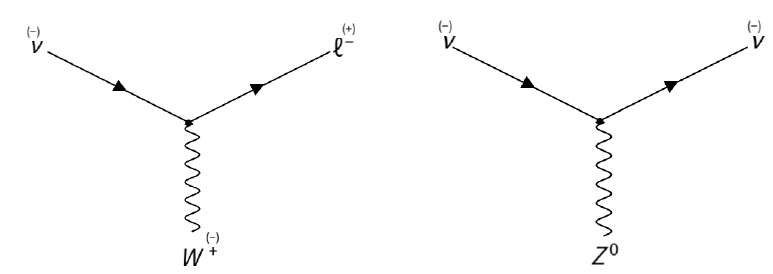
\includegraphics[width=\textwidth]{Figures/CC_NC.png}
    \caption{Feynman diagrams of charged-current (left) and neutral-current (right) neutrino interactions}
    \label{fig:CC_NC}
\end{figure}


One such interaction, and often the simplest interaction, is neutrino-electron elastic scattering ($\nu+e^{-} \rightarrow \nu+e^{-}$), which occurs when a neutrino scatters off an electron with a virtual vector boson being exchanged. hTis type of scattering is used in the detection of low energy neutrinos, primarily those from the sun \cite{RevModPhys.59.505}. Figure \ref{fig:elastic_scattering} shows the Feynman diagrams for this kind of interaction.

\begin{figure}
    \centering
    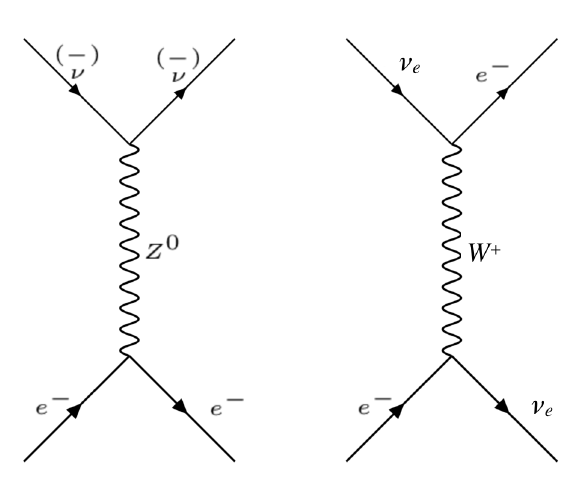
\includegraphics[width=0.6\textwidth]{Figures/elastic_scattering.png}
    \caption{Feynman diagrams of neutral-current (left) and charged-current (right) neutrino-electron scattering}
    \label{fig:elastic_scattering}
\end{figure}

There are multiple types of neutrino-nucleus interactions that occur which can be either charged current or neutral current interactions. These are given in order of momentum transfer ($q^2$), with the lowest neutrino energies producing quasi-elastic scattering for charged current interactions, and elastic scattering for neutral current interactions, up to deep inelastic scattering where the target nucleus breaks up. 

Starting off with the neutrino-nucleus interaction with the lowest $q^2$, the Feynman diagrams for NC elastic and CCQE interactions by a muon neutrino interacting with a neutron are shown in Figure \ref{fig:ncel_ccqe}. 

\begin{figure}
    \centering
    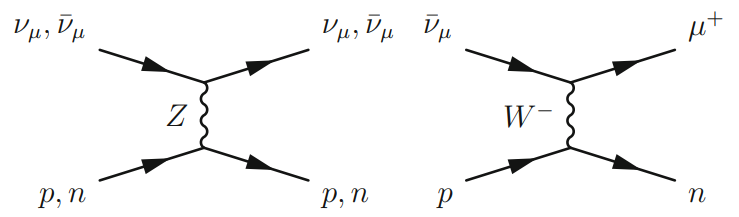
\includegraphics[width=0.6\textwidth]{Figures/ncel_ccqe.png}
    \caption{Feynman diagram for $\nu_{\mu}$ NC elastic scattering (left) and $\nu_{\mu}$ CCQE scattering (right)}
    \label{fig:ncel_ccqe}
\end{figure}

The type of interaction that occurs at higher neutrino energies,i.e. with more $q^2$ available is resonance production \cite{PhysRevD.69.014013}. Single mesons can also be produced via neutrino-nucleon reactions: these are mostly pions, but some kaons and eta particles can also be produced. Here a neutrino with a high enough energy interacts with and excites a nucleon, producing a resonant baryon which decays to a nucleon and a single pion (shown in Equation \ref{eq:resonant_pion}), where $N$ and $N'$ are nucleons.


\begin{align}
\nu_{l}+N \rightarrow l+N^{*}\label{eq:resonant_pion} \\
N^{*} \rightarrow \pi+N^{\prime} \notag
\end{align}


The resonant baryon produced during the reaction is usually a $\Delta(1232)$ resonance. 

Single pion final states can also be priduced by a neutrino which scatters off an entire nucleus (X), shown in Equation \ref{eq:single_pion_CC} for the charged current reactions and Equation \ref{eq:single_pion_NC} for neutral current reactions. 

\begin{equation}
\nu_{l}+X \rightarrow l^{-}+X+\pi^{+}, \quad \bar{\nu}_{l}+X \rightarrow l^{+}+X+\pi^{-}
\label{eq:single_pion_CC}
\end{equation}

\begin{equation}
\nu_{l}+X \rightarrow \nu_{l}+X+\pi^{0}, \quad \bar{\nu}_{l}+X \rightarrow \bar{\nu}_{l}+X+\pi^{0}
\label{eq:single_pion_NC}
\end{equation}

At higher energies (above 1 GeV), neutrino interactions can also produce kaons in the final state, due to the higher energies being able to produce strange quarks. 

At even higher energies and greater $q^2$, deep inelastic scattering is able to occur \cite{kulagin2007neutrino}. Deep inelastic scattering is a type of neutrino interaction where the neutrino scatters off a quark inside the proton or neutron involved in the exchange, via a W (CC) or Z (NC) boson (Equation \ref{eq:DIS_eq}), shown in Figure \ref{fig:CC_DIS}.


\begin{align}
&\nu_{l}+N \rightarrow l^{-}+X, \quad \bar{\nu}_{l}+N \rightarrow l^{+}+X(\mathrm{CC}) \label{eq:DIS_eq}\\
&\nu_{l}+N \rightarrow \nu_{l}+X, \quad \bar{\nu}_{l}+N \rightarrow \bar{\nu}_{l}+X(\mathrm{NC}) \notag
\end{align}


\begin{figure}
    \centering
    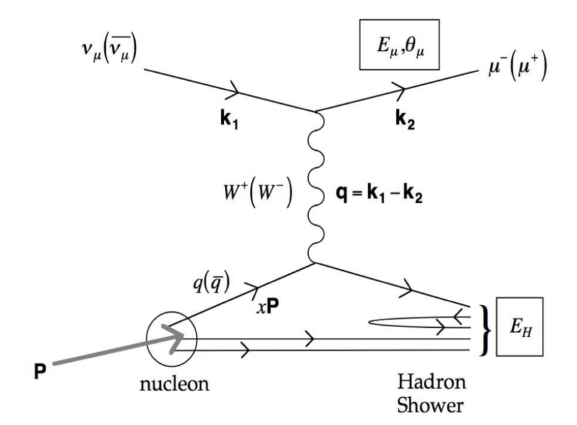
\includegraphics[width=0.7\textwidth]{Figures/CC_DIS.png}
    \caption{Feynman diagram for a charged current deep inelastic scattering interaction with an incoming muon neutrino}
    \label{fig:CC_DIS}
\end{figure}

The next two neutrino-nucleus interactions explained here are of particular relevance to the analysis in this thesis: inverse beta decay (IBD) and quasi-elastic scattering. 

Inverse beta decay is the reaction by which Cowan and Reines first detected electron antineutrinos: it is important at low energies: from the minimum energy for the reaction to take place ($E_{\nu}$ = 1.806 MeV) to tens of MeV \cite{oralbaev2016inverse}. Diffuse Supernova Neutrino Background and low energy antineutrinos produced from nuclear reactors can be detected via this process \cite{li2022prospects}. Figure \ref{fig:IBD_feynman} shows the Feynman diagram for this reaction. The neutron produced by this reaction is integral to the motivation behind the Gadolinium-doping upgrade to Super-Kamiokande, which will be explained in the next section.

\begin{figure}
    \centering
    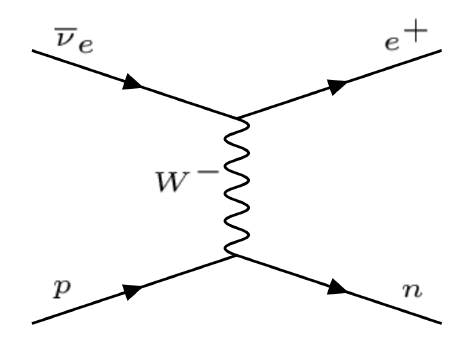
\includegraphics[width=0.7\textwidth]{Figures/IBD_feynman.png}
    \caption{Feynman diagram for the inverse beta decay reaction}
    \label{fig:IBD_feynman}
\end{figure}

Finally, we get to the type of interaction investigated in this thesis: quasi-elastic scattering. This makes up the majority of the neutrino-nucleus interaction cross-sections at the energy range from 100 MeV to ~2 GeV, and therefore vital for the study of neutrinos from long baseline neutrino experiments and also low energy atmospheric neutrinos \cite{wan2019measurement}. Equation \ref{eq:QE_reaction} shows the equations for both the charge current (CCQE) and neutral current (NCQE) version of this interaction where the incoming neutrino scatters off a nucleon.


\begin{align} 
\mathrm{CC}: \nu(k)+n(p) & \rightarrow l^{-}\left(k^{\prime}\right)+p\left(p^{\prime}\right) \label{eq:QE_reaction}\\
\bar{\nu}(k)+p(p) & \rightarrow l^{+}\left(k^{\prime}\right)+n\left(p^{\prime}\right) \notag\\
\mathrm{NC}: \nu(k)+N(p) & \rightarrow \quad \nu\left(k^{\prime}\right)+N\left(p^{\prime}\right) \notag \\
\bar{\nu}(k)+N(p) & \rightarrow \bar{\nu}\left(k^{\prime}\right)+N\left(p^{\prime}\right) \notag 
\end{align}



\begin{figure}
    \centering
    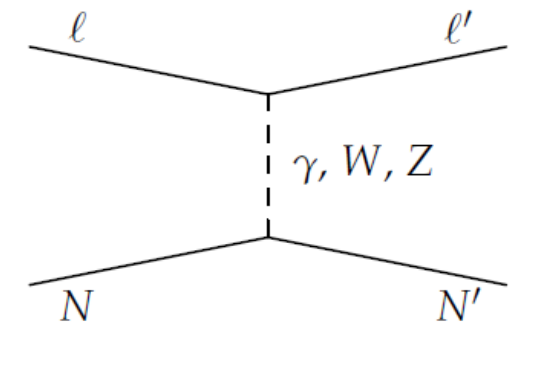
\includegraphics[width=0.7\textwidth]{Figures/QE_feynman.png}
    \caption{Feynman diagram for a quasi elastic scattering interaction off a nucleon}
    \label{fig:QE_reaction}
\end{figure}



As this analysis relates to the various properties of neutrons produced from NCQE interactions in Super-Kamiokande Gd, it is worth looking at the interactions where neutrons are produced inside the detector medium. In Water Cherenkov detectors, the incoming neutrino or anti-neutrino interacts with an ${ }^{16} \mathrm{O}$ nucleus, and at neutrino energies greater than 200 MeV, a nucleon is knocked out, as shown in Equation \ref{eq:nu_nucleon}.

\begin{align}
&\nu(\bar{\nu})+{ }^{16} \mathrm{O} \rightarrow \nu(\bar{\nu})+n+{ }^{15} \mathrm{O}^{*} \label{eq:nu_nucleon} \\
&\nu(\bar{\nu})+{ }^{16} \mathrm{O} \rightarrow \nu(\bar{\nu})+p+{ }^{15} \mathrm{~N}^{*} \notag
\end{align}


This interaction hapens in stages, where there is the initial reaction between the incoming neutrino and the specific nucleon inside the ${ }^{16} \mathrm{O}$ nucleus, hadronic final state interactions (FSI) inside the nucleus itself, and subsequent hadronic secondary interactions (SI) inside the detector medium. These are outlined in the schematic shown in Figure \ref{fig:FSI_SI}, with the primary interaction, taken as the CCQE reaction ($\bar{\nu}(k)+p(p) \rightarrow l^{+}\left(k^{\prime}\right)+n\left(p^{\prime}\right)$).
There are stages to neutrino-nucleus reactions, and for the CCQE reaction shown in Figure \ref{fig:FSI_SI}, there are three processes: the initial neutrino-nucleon reaction ($\bar{\nu}(k)+p(p) \rightarrow l^{+}\left(k^{\prime}\right)+n\left(p^{\prime}\right)$), the final state interaction (FSI) \cite{Golan_2012} inside the ${ }^{16} \mathrm{O}$ nucleus ($p+p \rightarrow p+n+\pi^{+}$), and the secondary (SI) interaction \cite{haigh2015results} in the detector medium ($n+{ }^{16} O \rightarrow n+n+{ }^{15} O^{*}$). All interactions inside the nucleus are referred to as hadronic final state interactions, and when they move through the detector medium and leave the target nucleus they are known as hadronic secondary interactions. 


\begin{figure}
    \centering
    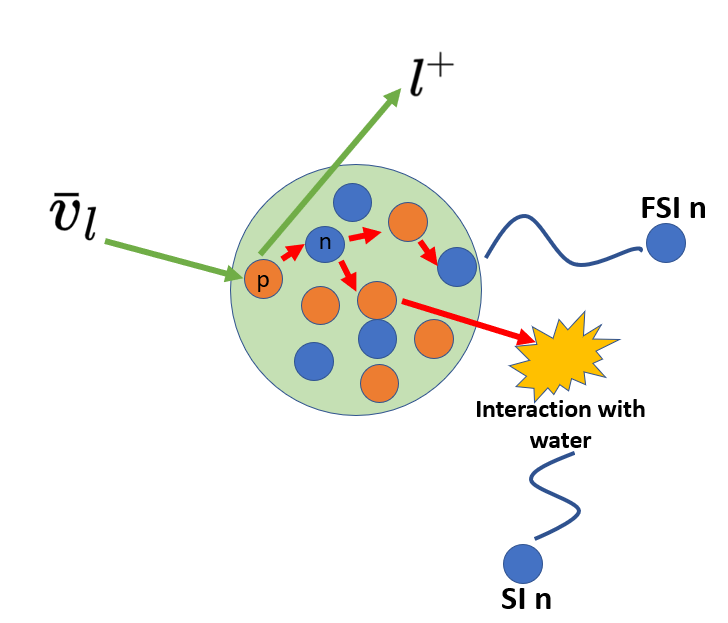
\includegraphics[width=0.7\textwidth]{Figures/fsi_schematic.png}
    \caption{Schematic of neutron production following the interaction of neutrino with a nucleon inside an ${ }^{16} \mathrm{O}$ and the resulting FSI and SI interactions in the detector medium.}
    \label{fig:FSI_SI}
\end{figure}



\subsection{Diffuse Supernova Neutrino Background}

A key feature of the analysis presented in this thesis is that it is an investigation into the significant background of the signal for DSNB \cite{malek2003search}. It is therefore important to state and understand the process behind the production of supernova relic neutrinos in order to get a firm handle on the motivation behind this analysis. 

\subsubsection{Supernovae Classification}
Supernovae occur when a star with a mass around eight times the mass of our sun explodes, and in a galaxy these occur only a few times in a century \cite{van1991supernova}. Supernovae are classified into different types: Type 1a, Type 1b, Type 1c and Type II \cite{turatto2003classification}. The classification of supernovae are determined by looking at the spectral lines in the light emitted from these supernovae. Table \ref{table:supernova_classification} shows how these supernovae are classed and which spectral line elements are associated with each class. 

\begin{table}
\centering
\begin{tabular}{||c c||} 
    \hline
    Supernova Classification & Element lines present in spectra \\ 
    \hline 
    Type 1a & No hydrogen, silicon  \\ 
    \hline
    Type 1b & No hydrogen, no silicon, helium  \\
    \hline
    Type 1c & No hydrogen, no silicon, no helium  \\
    \hline
    Type II & Hydrogen  \\
    \hline 
\end{tabular}
\caption{Supernovae classification along with the element lines present in their spectra \cite{Gal_Yam_2017}.}
\label{table:supernova_classification}
\end{table}

The kinetic energy of a supernova is ~$10^{44}$ J, and 99 \% of the energy from core-collapse supernovae (CCSN) are released in the the form of neutrinos \cite{scholberg2012supernova}. Unlike Type 1a supernovae which are usually thermonuclear supernovae, Type 1b, Type 1c and Type II are core-collapse supernovae, from which more neutrinos are emitted which is why these types of supernovae are of more interest. 

\subsubsection{Core-Collapse Supernovae Mechanism}

Using the pressure produced by the process of nuclear fusion, a star is able to support itself against gravotational collapse. During the proton-proton chain reaction, hydrogen will fuse to produce helium and once temperatures and pressures are high enough, helium fusion will occur. After all the helium in the core is used up in the fusion process, the star will contract until the pressure and temperatures get even higher, allowing more massive nuclei to fuse. This reaction will carry on until iron nuclei are produced, this being the element with the highest binding energy, causing the fusion to stop \cite{couch2017mechanism}.
\newline
As more and more iron accumulates in the core of the star, the density and temperature of the core will increase, and these higher energy electrons will increase the rate of electron capture on protons that will occur in the iron nuclei \cite{fryer2019gamma}. This will cause a reduction in the electron degeneracy pressure, which is further enhanced by the breakdown of the iron nuclei which occurs at higher temperatues when gamma rays interact with them. The degeneracy pressure is no longer greater than the gravitational forces acting inwards, and gravitational core collapse occurs \cite{ebinger2017global}. 
\newline
The point at which in the core the neutrino mean free paths become become approximately the same size as the proto-neutron star is called the ``neutrinosphere" \cite{PhysRevD.101.023018}.  Figure \ref{fig:neutrinosphere} shows the formation of a proto-neutron star (PNS) and the neutrino flux and neutrinosphere produced by the core-collapse mechanism. 

\begin{figure}
    \centering
    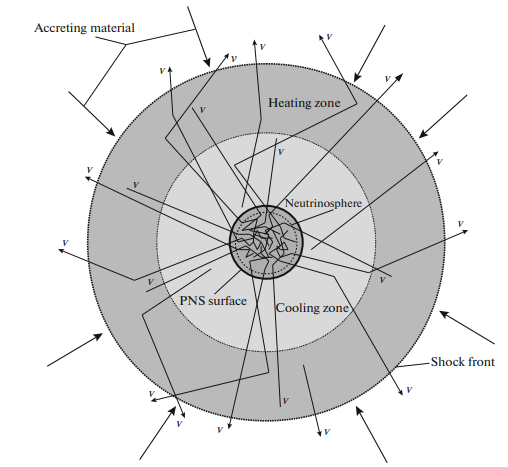
\includegraphics[width=0.7\textwidth]{Figures/neutrinosphere.png}
    \caption{Schematic showing core collapse of a star, and the resultant shockwave and neutrino production}
    \label{fig:neutrinosphere}
\end{figure}


The radius of the neutrinosphere becomes as large as that of the inner core of the star, when the inner core of the star reaches a density of ~$10^{11} gcm^{-3}$, and the electron neutrinos produced from electron capture become unable to escape. Gravitational collapse of the star continues until the inner core reaches nuclear density, at which point a shock wave is produced due to the repulsive force between nuclei \cite{PhysRevLett.60.1999}. 
\newline

When this shock wave reaches the neutrinosphere, neutrino emission begins, which lasts less than 10 milliseconds. After this shockwave passes, nucleons and electrons fall back onto the proto-neutron star which heats it up. This causes neutrinos of all flavours to be produced via pair production and electron capture. This is called the ``accretion phase" \cite{pajkos2019features}. Due to this expulsion of neutrinos the shock wave loses energy, but it is revived through matter behind the shock wave being heated by neutrino absorption from the proto-neutron star region \cite{pascal2022proto}. The mechanism for this shown in Figure \ref{fig:ccsn_mechanism}, where the shockwave produced depends on antineutrinos being absorbed by the dense post-shock gas. 
\newline

\begin{figure}
    \centering
    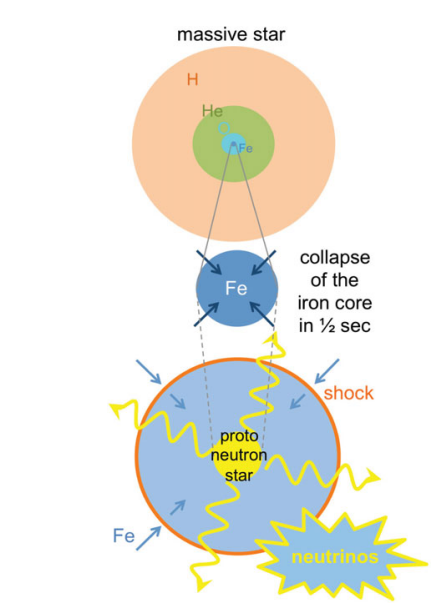
\includegraphics[width=0.7\textwidth]{Figures/ccsn_mechanism.png}
    \caption{Schematic showing core collapse of a star, and the resultant shockwave and neutrino production}
    \label{fig:ccsn_mechanism}
\end{figure}

After the shock wave is revived, if it has enough energy to blow off the outer layer of matter a supernova occurs. Then, depending on the mass of the PNS, it cools to either become a neutron star or a black hole \cite{o2011black}. If the shock wave energy is not high enough to blow off the outer layer of matter, the accretion phase continues until a black hole is formed.
\newline

The energy of the emitted neutrinos depend on their flavour - neutrinos emitted from a deeper layer inside the supernova will be higher in temperature and therefore have a higher energy. For electron neutrinos and electron anti-neutrinos, the dominant interactions are charged current interactions with nucleons. Due to the number of neutrons in a proto-neutron star greatly outnumbering the number of protons, the interaction involving $\nu_{e}$ will be far more efficient than those involving $\nu_{\bar{e}}$, meaning the neutrinosphere for $\nu_{\bar{e}}$ is smaller than for $\nu_{e}$, so they are emitted from the PNS with greater energies. 

Due to there being no charged current interactions involving muon neutrinos in the medium, they are involved instead in neutral current reactions, including Bremsstrahlung, neutrino-pair annhilation, and electron-positron pair annhilation \cite{betranhandy2020impact}. Due to only undergoing these reactions their neutrinosphere is even smaller than that of their electron neutrino and electron anti-neutrino counterparts, therefore being emitted wih even higher energies \cite{nagakura_non-thermal_2021}. Figure \ref{fig:ccsn_nu_flavor_energy} shows the luminosity (top panels) and average energy (bottom panels) for three different neutrino flavours as a function of time for the neutronisation phase (left), accretion phase (centre) and cooling phase (right). Taken from \cite{chakraborty_observing_2014}.

\begin{figure}
    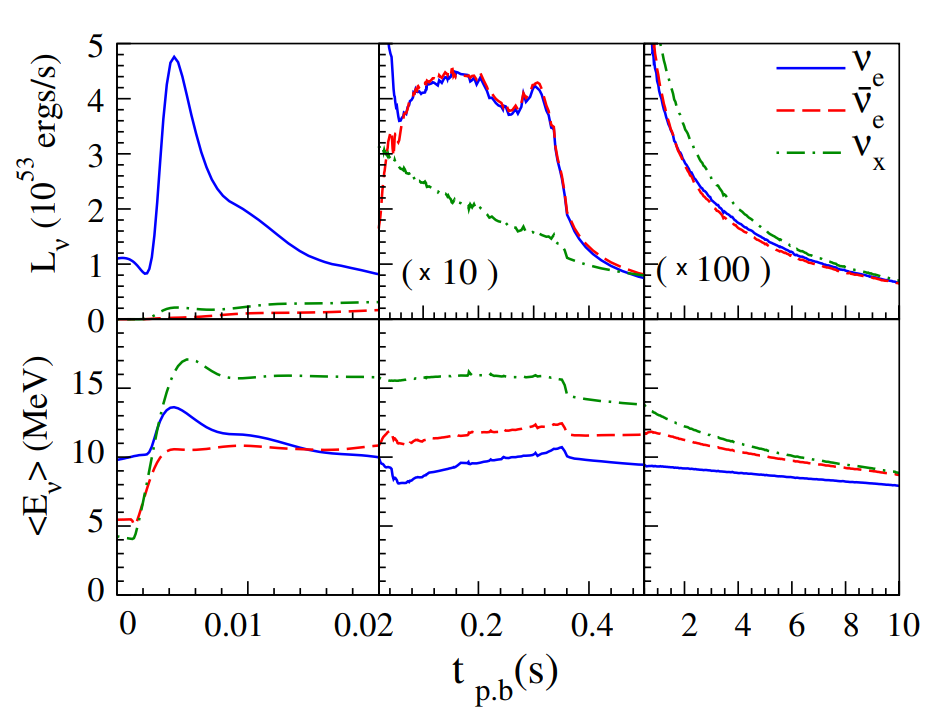
\includegraphics[width=\textwidth]{Figures/ccsn_nu_flavor_energy.png}
    \caption{Luminosity (top panels) and average energy (bottom panels) for three different neutrino flavours as a function of time for the neutronisation phase (left), accretion phase (centre) and cooling phase (right). Taken from \cite{chakraborty_observing_2014}. }
    \label{fig:ccsn_nu_flavor_energy}
\end{figure}



Kamiokande-II observed neutrinos produced from a supernova, later named 1987A, in the Large Magellenic Cloud. These neutrinos were also observed by the Baskan Neutrino Observatory and the Irvine-Michigan-Brookhaven detector (IMB) \cite{hirata_observation_1987}. The neutrinos detcted from 1987A were detected via the inverse beta decay (IBD) interaction (shown in Figure \ref{fig:IBD_feynman}), as opposed to the electron elastic scattering, CC interaction with ${ }^{16} \mathrm{O}$ or NC interaction with  ${ }^{16} \mathrm{O}$ channels. The positron from this reaction is what is searched for, and these positrons are produced isotropically within the detector. A neutrino burst search from SN1987A was carried out on the data run which ran continuously between 16:09 21 February 1987 to 07:31 24th February 1987 JST \cite{Hirata:1988ad}.

The event selection criteria for a supernova neutrino event were as follows: firstly, the total number of photoelectrons per event should be less than 170, as this corresponds to an electron with an energy of 50 MeV, and the neutrinos released from a supernovae have a typical energy of the order of 10 MeV. Secondly, the total number of electrons in the outer detector per event needed to be less than 30, in order for the event to be considered fully contained, and finally, the time between previous events has to be greater than 20 $\mu$sec, in order to avoid electrons produced from Michel electrons. Figure \ref{fig:1987A_events} shows the time-sequence of all low-energy events. If the neutrinos were to show up in Kamiokande-II, they would arive in a cluster lasting of order 10s, so intervals of 10 seconds were used to seacrh for clusters of events. In order to classify the event as a supernova neutrino candidate, the event had to be registered by atleast 30 PMTs, and 6 events were found in the first 10s interval which satisfied this, and 2 events in the next 10s interval. A second search was performed on a larger data sample of 42.9 days, from 9th of January to 25th of February 1987, and no other supernova neutrino burst candidates were found. The first two events shown in Figure \ref{fig:1987A_events} also correlate in angle to the direction of 1987A. As a result, this was considered detection of a genuine supernova neutrino burst, and was the first direct observation of this in neutrino astronomy. 

\begin{figure}
    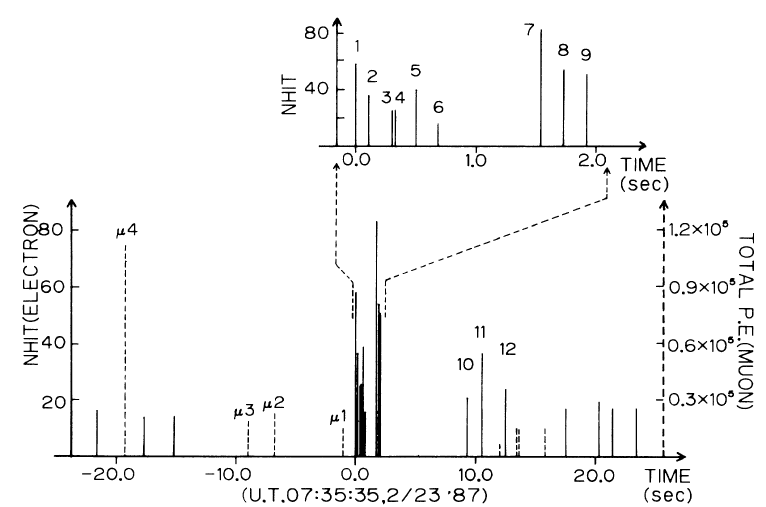
\includegraphics[width=\textwidth]{Figures/1987A_events.png}
    \caption{Events detected centered on 16:35:35 JST,  where the solid lines are the number of hit PMTs and dashed lines are muon events. The zoomed in plot in the top-right shows an expanded version of the 0.0 - 2.0 second time scale.  }
    \label{fig:1987A_events}
\end{figure}

Due to neutrinos carrying away 99\% of the energy produced by supernovae, they are the most important signal a supernova can produce, and can be used for finding out when the supernova explosion actually happened - due to neutrinos leaving the supernovae immediately while gamma rays from the the explosion can only leave the supernova when the shock wave reaches the surface of the star \cite{bethe_supernova_1990}.

The supernova relic neutrinos emitted from all past CCSN are accumulated and form an everpresent background due to the fact that neutrinos only weakly interact with matter. The total flux of this neutrino background has been theoretically predicted and is called the ``diffuse supernova neutrino background" (DSNB). When calculating the total DSNB flux, the redshift caused by the expansion of the universe needs to be taken into account.

Equation \ref{eq:SRNflux} gives the differential of the DSNB flux with respect to the DSNB energy at Earth \cite{beacom2010diffuse}.

\begin{equation}
\mathrm{d} n_{\nu}\left(E_{\nu}\right)=R_{\mathrm{SN}}(z) \frac{\mathrm{d} t}{\mathrm{~d} z} \mathrm{~d} z \frac{\mathrm{d} N_{\nu}\left(E_{\nu}^{\prime}\right)}{\mathrm{d} E_{\nu}^{\prime}}(1+z) \mathrm{d} E_{\nu}
\label{eq:SRNflux}
\end{equation}

Here $E_{\nu}^{\prime}=(1+z) E_{\nu}$ is the energy of neutrinos at a certain redshift $z$, $R_{\mathrm{SN}}(z)$ is the supernova rate at a comoving volume at $z$, $\mathrm{d} N_{\nu} / \mathrm{d} E_{\nu}$ is the number spectrum of neutrinos emitted by one supernova explosion, and $(1+z)^{-3}$ is the expansion of the universe factor. The relationship between redshift and time ($dt/dz$), is given by the Friedmann equation (Equation \ref{eq:friedmann}), where $H_{0}$ is the Hubble constant, $\Omega_{m}$ is the matter density and $\Omega_{\Lambda}$ is the cosmological constant \cite{ando_relic_2004}.

\begin{equation}
\frac{\mathrm{d} z}{\mathrm{~d} t}=-H_{0}(1+z) \sqrt{\Omega_{\mathrm{m}}(1+z)^{3}+\Omega_{\Lambda}}
\label{eq:friedmann}
\end{equation}

It is worth reviewing the lastest searches from Super-Kamiokande for DSNB neutrinos, and the limit on the flux prediction from different Super-Kamiokande phases. While Figure \ref{fig:DSNBenergy} shows that the majority of DSNB neutrinos have an energy below 10 MeV, due to massive backgrounds these DSNB are hard to detect, so Super-Kamiokande therefore searches for the DSNB signal in the order of 10 MeV. As mentioned previously the main detection channel is inverse-beta decay, with the prompt signal being the emitted positron and the delayed signal constituting of the photon emission from neutron capture. Up to and including now, there has been no DSNB signal evidence but upper-limits on the flux have been set from both KamLAND and from Super-Kamiokande phases I-IV, shown in Figure \ref{fig:DSNBlimit}.


\begin{figure}
    \centering
    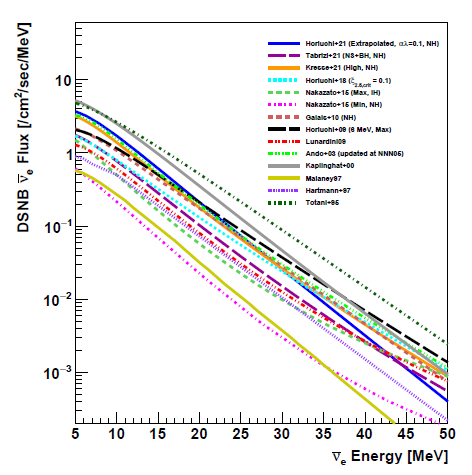
\includegraphics[width=0.5\textwidth]{Figures/DSNB_energy.png}
    \caption{DSNB flux against neutrino energy for various theoretical models, "NH'' and "IH'' are the normal and inverted mass hierchies respectively}
    \label{fig:DSNBenergy}
\end{figure}

\begin{figure}
    \centering
    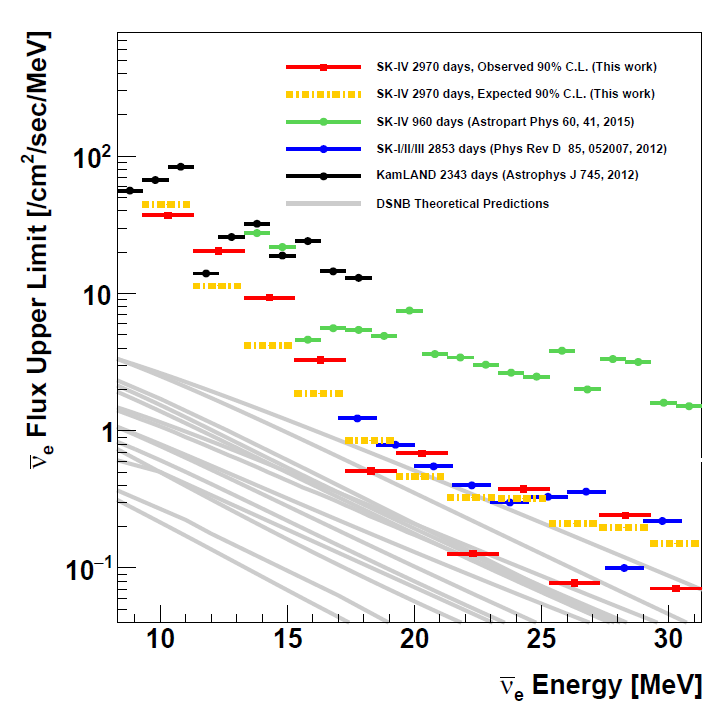
\includegraphics[width=0.5\textwidth]{Figures/DSNBlimit.png}
    \caption{The 90\% C.L. for observed and expected upper limits on the electron antineutrino flux from SK-I - SK-IV and KamLAND, with the theoretical predictions in Figure \ref{fig:DSNBenergy} shown in grey.}
    \label{fig:DSNBlimit}
\end{figure}


Regarding important backgrounds to the DSNB signal, below neutrino energies of 15 MeV NCQE interactions from atmospheric neutrinos form the main background to DSNB searches. The importance of this background motivates the analysis in this thesis: by measuring the NCQE interaction using T2K beam neutrinos \cite{abe2021diffuse}, the large uncertainty of this interaction in the low energy region can be reduced due to the reason that the atmospheric neutrino energy region is similar to that of the T2K beam energy region. The differential cross section of the neutral-current elastic interaction of a neutrino on a free proton or neutron can be written as shown in Equation \ref{eq:NCQExsec}. 

\begin{equation}
\frac{d \sigma^{\nu(\bar{\nu})}}{d q^{2}}=\frac{M^{2} G_{F}^{2}}{8 \pi E_{\nu}^{2}}\left\{A\left(q^{2}\right) \pm B\left(q^{2}\right) \frac{s-u}{M^{2}}+c\left(q^{2}\right) \frac{(s-u)^{2}}{M^{4}}\right\}
\label{eq:NCQExsec}
\end{equation}
    
where $E_{\nu}$ is the initial neutrino or antineutrino energy, $M$ is the mass of the nucleon, $G_{F}$ is the Fermi coupling constant \cite{van2000precise}, $s$ and $u$ are the Mandelstam variables, and $q$ is the transfer of four momentum between between incoming (anti)neutrinos and outgoing (anti)neutrinos. Depending on whether it is an incoming neutrino or antineutrino, there is either a plus or a minus between the A and B terms. A,B and C are terms which are made up of form factors specific to neutral current interactions.


\subsection{Physics motivation behind Super-Kamiokande Gadolinium Upgrade}

Due to the large cross section of the IBD interaction, IBD events constitute about 88\% of the total number of events in the detector \cite{marti_evaluation_2020}. With efficient neutron tagging in Super-Kamiokande, the backgrounds (charged current interactions and muon spallation) in the search for DSNB flux neutrinos would be largely reduced. The neutral current quasielastic (NCQE) background would still remain due to the way the gamma rays arising from neutron capture mimic the signal of the inverse beta decay (IBD) reactions: a schematic of both NCQE and IBD reactions are shown in Figure \ref{fig:NCQE_IBD}. The measurement of the NCQE interactions using T2K beam flux can aid in understanding this background more due to the T2K flux peak being near the atmospheric neutrino flux peak (~600 MeV). 


\begin{figure}
    \centering
    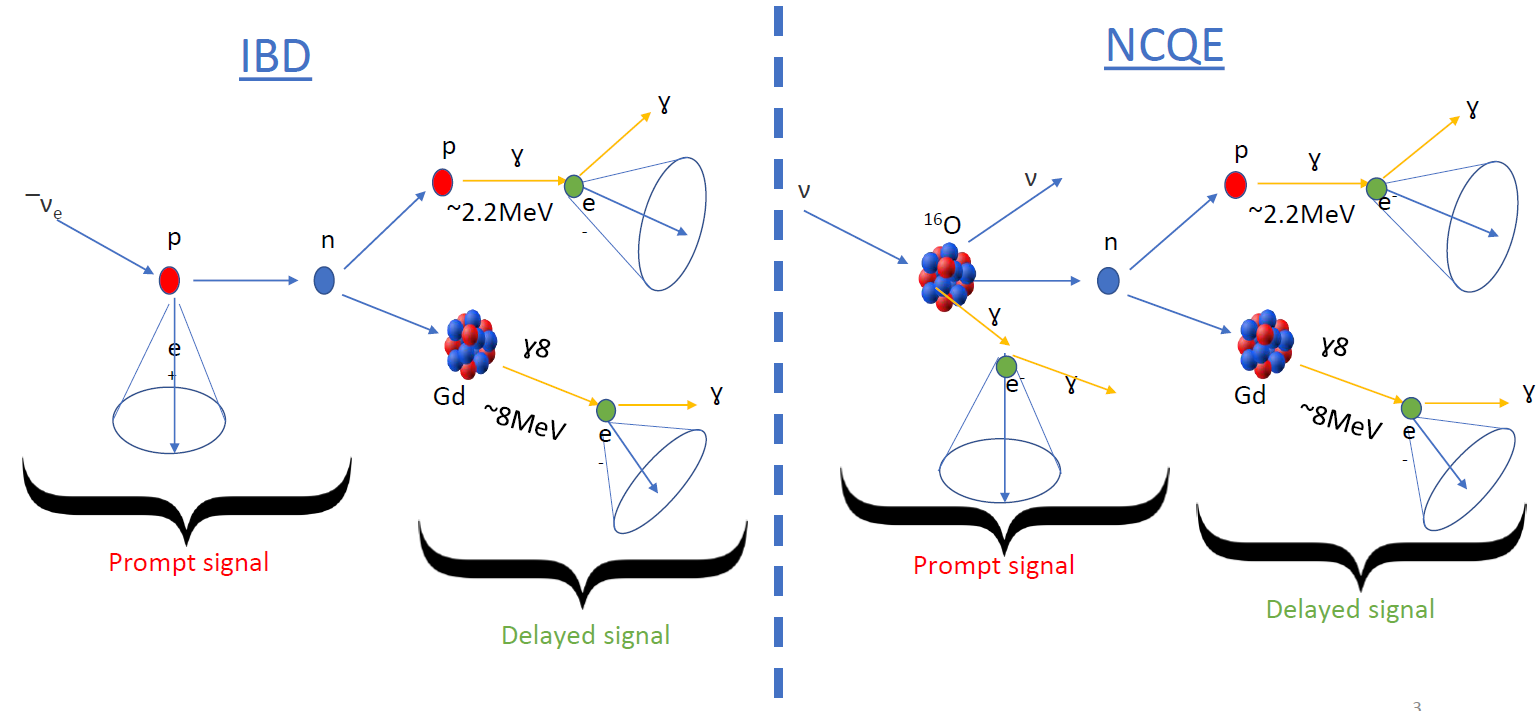
\includegraphics[width=\textwidth]{Figures/schematic.png}
\caption{Schematic showing the IBD and NCQE interaction mechanisms}
\label{fig:NCQE_IBD}
\end{figure}


Efficient neutron tagging aids information about neutrino energy and neutrino interaction type, and when it comes to studying atmospheric neutrino oscillations, accurate neutrino energy reconstruction is particularly important. Figure \ref{fig:atm_nu_energy} shows the fraction of non-visible energy as a function of the number of tagged neutrons from simulations of atmospheric neutrino interactions at Super-Kamiokande. Here $E_{\nu}$ is the energy of the atmospheric neutrino and $E_{vis}$ is the energy that is reconstructed from charged particles. Due to these neutrinos interacting with nuclei in the detector, more neutrons are produced, and with efficient neutron tagging on gadolinium the neutrino energy can be properly reconstructed. 

\begin{figure}
    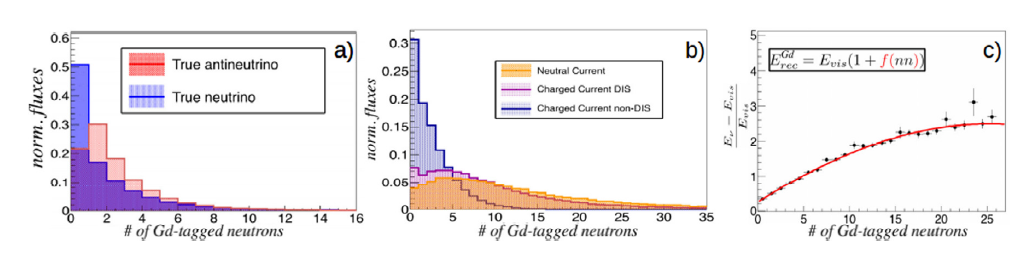
\includegraphics[width=\textwidth]{Figures/atm_recon_energy.png}
\caption{MC study of (a) neutron multiplicity production for $\nu$ and ${\bar{\nu}}$, (b) neutral current, charged current and deep and non-deep inelastic scattering, (c) the correction to the visible energy as a function of neutrino multiplicity. Taken from \cite{marti_evaluation_2020}.}
\label{fig:atm_nu_energy}
\end{figure}



The ideal goal of this analysis is to complement prior analyses which investigate the NCQE cross-section and analyses which produce neutron multiplicity distributions for NCQE interactions, with the added benefit of comparisons to Run 11 T2K data, which brings with it the first beam events with gadolinium in the far detector. The emphasis on the distributions of neutrons in this thesis and the methods of neutron tagging used are of increasing interest due to the fact that the main purpose behind adding Gadolinium to the detector is to make these neutron captures more visible. Futhermore, in Chapter 8, an estimate of the DSNB NCQE background is made, with an error stemming from the value of the neutron tagging efficiency and systematic error on this efficiency calculated in Chapter 6 and Chapter 7 of this thesis.


